\documentclass[12pt]{article}
\usepackage{caption}
\usepackage{subcaption}
\usepackage{graphicx}
\usepackage{amsmath}
\usepackage{hyperref}

\begin{document}

\begin{titlepage}
    \begin{center}
        \huge
        Elliptic Filter\\Design Report
        \vfill
        \large
        Student Details:\\\vspace{3pt}
        Name: Kanak Yadav\\\vspace{3pt}
        Roll No: 20D070044\\\vspace{3pt}
        Filter Number: 55\\\vspace{3pt}
        Group Number: 37\\\vspace{60pt}
        \vfill
    \end{center}
\end{titlepage}

\section{Bandpass Filter Design}
\subsection{Un-normalized Discrete Time Filter}
\[q(m) = r(m) = 5\]
Substituting the values of q(m) and r(m), we get
\begin{align*}
    BL(m) &= 10 + 5(5) + 13(5)\\
    &= 100,\\
    BH(m) &= 100 + 75\\
    &= 175.
\end{align*}
Thus, the passband edges are:
\begin{align*}
    f_{p1} &= 100 kHz,\\
    f_{p2} &= 175 kHz.
\end{align*}
The transition bandwidth is given to be\[\Delta_f = 5 kHz.\]
Thus, the stopband edges are:
\begin{align*}
    f_{s1} &= f_{p1} - \Delta_f = 95 kHz,\\
    f_{s2} &= f_{p1} + \Delta_f = 180 kHz.
\end{align*}

Now we can state the specifications of the discrete-time bandpass filter.
\newline
\hline
\vspace{10pt}
\textbf{Specifications:}
\begin{itemize}
    \item Passband: 100 kHz to 175 kHz,
    \item Stopband: 0 to 95 kHz and 180 kHz to 300 kHz (since $f_s$ = 600 kHz),
    \item Passband and Stopband tolerance: 0.15,
    \item Passband and Stopband nature: Rippled.
\end{itemize}
\hline

\subsection{Normalized Digital Filter}
Given that our signal of interest is bandlimited to
\[f_b = 280 kHz,\]
to satisfy the Nyquist Criterion,
\[f_s > 2 f_b = 560 kHz.\]
Given sampling frequency is
\[f_s = 600 kHz > 560 kHz.\]
Hence, the Nyquist criterion is satisfied.

For normalizing the frequencies, we need to make the sampling frequency map to $2\pi$. Thus,
\[\omega = \frac{2\pi f}{f_s}\]
This gives us the normalized digital frequencies as follows:
\begin{table}[h]
    \centering
    \begin{tabular}{|c|c|}\hline
         Discrete time frequency&Normalized digital frequency\\
         $f$ (kHz)&$\omega$ (radians)\\\hline
         0&0\\\hline
         95&$\omega_{s1}$ = 0.9948377\\\hline
         100&$\omega_{p1}$ = 1.0471976\\\hline
         175&$\omega_{p2}$ = 1.8325957\\\hline
         180&$\omega_{s2}$ = 1.8849556\\\hline
         300&$\pi$\\\hline
    \end{tabular}
    \caption{Normalizing frequency.}
    \label{tab:1}
\end{table}

Now we can state the specifications of the digital bandpass filter.
\newline
\hline
\vspace{10pt}
\textbf{Specifications:}
\begin{itemize}
    \item Passband: 1.0471976 to 1.8325957,
    \item Stopband: 0 to 0.9948377 and 1.8849556 to  $\pi$,
    \item Passband and Stopband tolerance: 0.15,
    \item Passband and Stopband nature: Rippled.
\end{itemize}
\hline

\subsection{Analog Bandpass Filter}
For converting the normalized digital specifications to the specifications for an analog filter of the same type (bandpass), we use the bilinear transformation:
\[s = \frac{1-z^{-1}}{1+z^{-1}},\]
substituting the values of s and z, we get
\begin{align*}
    j\Omega &= \frac{1-e^{-j\omega}}{1+e^{-j\omega}} = \frac{e^{j\omega/2}-e^{-j\omega/2}}{e^{+j\omega/2}+e^{-j\omega/2}}\\
    &= \frac{2j\sin(\omega/2)}{2\cos(\omega/2)} = j\tan(\omega/2)\\
    \Omega &= \tan(\omega/2)
\end{align*}
This gives us the analog bandpass frequencies as:
\begin{table}[h]
    \centering
    \begin{tabular}{|c|c|}\hline
         Normalized digital frequency&Analog frequency\\
         $\omega$ (radians)&$\Omega$\\\hline
         0&0\\\hline
         0.9948377&$\Omega_{s1}$ = 0.5429557\\\hline
         1.0471976&$\Omega_{p1}$ = 0.5773503\\\hline
         1.8325957&$\Omega_{p2}$ = 1.3032254\\\hline
         1.8849556&$\Omega_{s2}$ = 1.3763819\\\hline
         $\pi$&$\infty$\\\hline
    \end{tabular}
    \caption{Applying the bilinear transformation.}
    \label{tab:2}
\end{table}

Now we can state the specifications of the digital bandpass filter.
\newline
\hline
\vspace{10pt}
\textbf{Specifications:}
\begin{itemize}
    \item Passband: 0.5773503 to 1.3032254,
    \item Stopband: 0 to 0.5429557 and 1.3763819 to  $\infty$,
    \item Passband and Stopband tolerance: 0.15,
    \item Passband and Stopband nature: Rippled.
\end{itemize}
\hline

\subsection{Frequency Transformation}
We need to employ a frequency transformation to convert our bandpass filter specifications into those of a lowpass filter. For this, we use the frequency transformation derived from the impedance of a series LC circuit:
\[s_L = \frac{s^2 + \Omega_0^2}{Bs},\]
where the subscript L stands for Lowpass. $\Omega_0$ is the resonant frequency and B is the bandwidth of the series LC circuit. Substituting the values of s$_L$ and s, we get
\begin{align*}
    j\Omega_L &= \frac{(j\Omega)^2 + \Omega_0^2}{B(j\Omega)} = \frac{1}{j}\frac{(-\Omega^2 + \Omega_0^2)}{B\Omega}\\
    &= -j\frac{(-\Omega^2 + \Omega_0^2)}{B\Omega} = j\frac{(\Omega^2 - \Omega_0^2)}{B\Omega}\\
    \Omega_L &= \frac{\Omega^2 - \Omega_0^2}{B\Omega}
\end{align*}
Now, we have two degrees of freedom, $\Omega_0$ and B. We also decide to follow the convention that the passband edge of the lowpass filter, in both the positive and negative half of the $\Omega_L$ axis, has a magnitude of one. In other words, we want $\Omega_{p1}$ and $\Omega_{p2}$ to map to -1 and +1 respectively on the $\Omega_L$ axis. To achieve this, we solve the following two equations
\[-1 = \frac{\Omega_{p1}^2 - \Omega_0^2}{B\Omega_{p1}}\]
and
\[+1 = \frac{\Omega_{p2}^2 - \Omega_0^2}{B\Omega_{p2}}\]
By equating $\Omega_0^2$ we get
\begin{align*}
    \Omega_{p1}^2 + B\Omega_{p1} &= \Omega_{p2}^2 - B\Omega_{p2}\\
    B(\Omega_{p2} + \Omega_{p1}) &= \Omega_{p2}^2 - \Omega_{p1}^2\\
    B &= \Omega_{p2} - \Omega_{p1}
\end{align*}
Substituting the value of B, we get
\begin{align*}
    \Omega_0^2 &= \Omega_{p1}^2 + (\Omega_{p2} - \Omega_{p1})\Omega_{p1}\\
    \Omega_0^2 &= \Omega_{p1}^2 + \Omega_{p2}\Omega_{p1} - \Omega_{p1}^2 = \Omega_{p2}\Omega_{p1}\\
    \Omega_0 &= \sqrt{\Omega_{p2}\Omega_{p1}}
\end{align*}
By substituting the value of $\Omega_{p1}$ and $\Omega_{p2}$, we get
\begin{align*}
    B &= 1.3032254 - 0.5773503 = 0.7258751\\
    \Omega_0 &= \sqrt{(1.3032254)(0.5773503)} = \sqrt{0.7524175} \approx 0.8674200
\end{align*}
\hline
\vspace{10pt}
\textbf{Transformation and Parameters}
\begin{itemize}
    \item Transformation:\[\Omega_L = \frac{\Omega^2 - \Omega_0^2}{B\Omega}\]
    \item Parameters:
    \begin{itemize}
        \item $\Omega_0$ = 0.8674200,
        \item B = 0.7258751
    \end{itemize}
\end{itemize}
\hline
\newpage
\subsection{Analog Lowpass Filter}
Substituting the values of $\Omega_o$ and B, we get the frequency transformation to be employed as:
\[\Omega_L = \frac{\Omega^2 - (0.7524175)}{(0.7258751)\Omega}\]
This gives us the analog lowpass frequencies as:
\begin{table}[h]
    \centering
    \begin{tabular}{|c|c|}\hline
         Analog frequency&Analog Lowpass Frequency\\
         $\Omega$ &$\Omega_L$\\\hline
         0$^+$&$-\infty$\\\hline
         0.5429557&$\Omega_{Ls1}$ = -1.1611157\\\hline
         0.5773503&$\Omega_{Lp1}$ = -1\\\hline
         1.3032254&$\Omega_{Lp2}$ = 1\\\hline
         1.3763819&$\Omega_{Ls2}$ = 1.1430597\\\hline
         $\infty$&$\infty$\\\hline
    \end{tabular}
    \caption{Analog frequency transformation.}
    \label{tab:3}
\end{table}

The passband edge of the lowpass filter was specified to be one while employing the frequency transformation but, the stopband edge now has two possible values of which, we choose the more stringent value (the value with a smaller magnitude) since satisfying the stronger specifications will automatically satisfy the weaker specifications. Thus
\begin{align*}
    \Omega_p &= 1\\
    \Omega_s &= min(abs(\Omega_{Ls1}), abs(\Omega_{Ls1}))\\
    &= min(1.1611157, 1.1430597)\\
    \Omega_s &= 1.1430597
\end{align*}

Now we can state the specifications of the analog lowpass filter.
\newline
\hline
\vspace{10pt}
\textbf{Specifications:}
\begin{itemize}
    \item Passband: 0 to 1,
    \item Stopband: 1.1430597 to  $\infty$,
    \item Passband and Stopband tolerance: 0.15,
    \item Passband and Stopband nature: Monotonic.
\end{itemize}
\hline

\subsection{Elliptic Analog Lowpass Transfer Function}
The first step was finding the poles and zeros of the Elliptic analog lowpass transfer function using the functions provided in MATLAB.
\[N = 4,\]
\[\text{poles} = -0.0310 + j0.9995, -0.3536 + j0.7071,\]
\[\text{zeros} = j1.0639, j1.7690.\]
Then, the Transfer function can be obtained using these poles and zeros and their complex conjugates.

\begin{figure}[h]
    \centering
    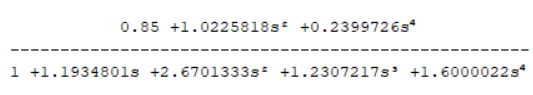
\includegraphics{h_lpf_bp.png}
    \caption{Screenshot from SCILAB Console.}
\end{figure}
Lowpass transfer function frequency response:

\begin{figure}[h]
    \begin{minipage}{0.49\linewidth}
        \centering
        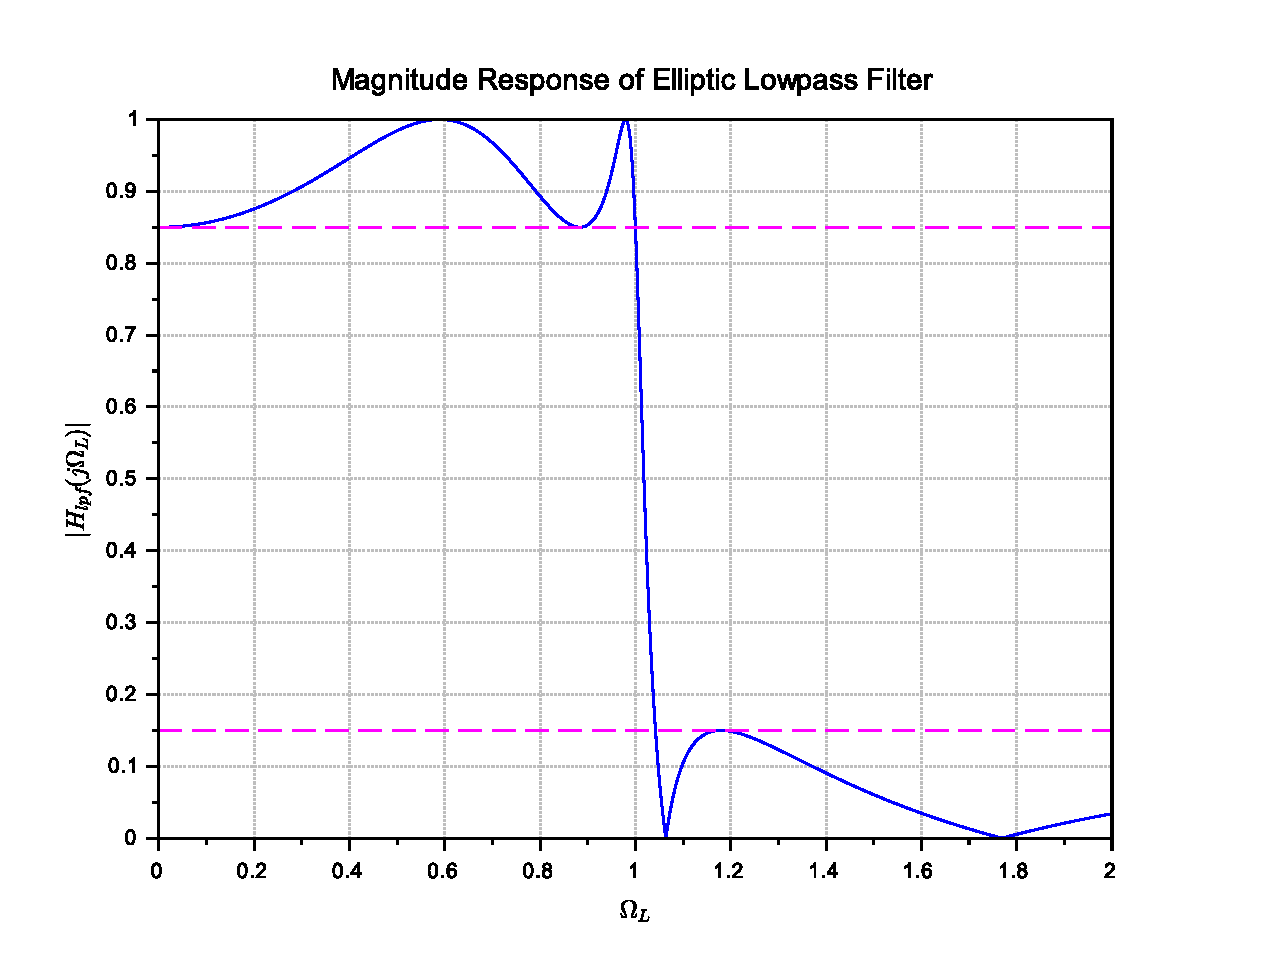
\includegraphics[scale=0.36]{mag_lpf_bp.pdf}
    \end{minipage}
    \begin{minipage}{0.49\linewidth}
        \centering
        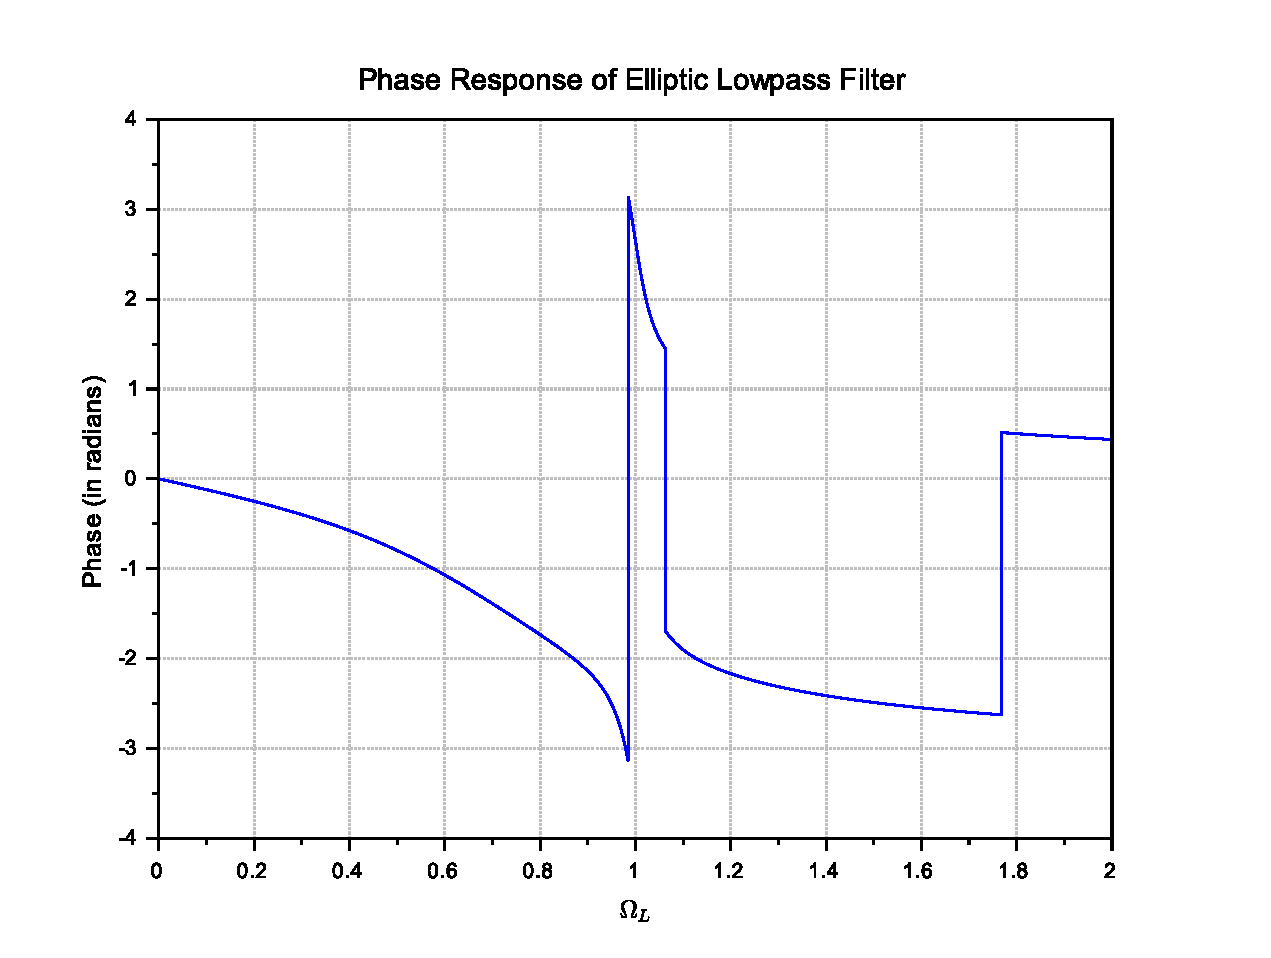
\includegraphics[scale=0.36]{phase_lpf_bp.pdf}
    \end{minipage}
\end{figure}
\newpage
\subsection{Analog Bandpass Transfer Function}
This can be obtained by replacing s$_\text{L}$ with F(s), the frequency transformation that we had employed earlier:
\[s_L \leftarrow F(s) = \frac{s^2 + \Omega_0^2}{Bs}\]
\textbf{H$_{\text{analog, BPF}}\text{(s)}$}
\begin{figure}[h]
    \centering
    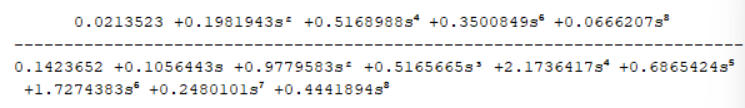
\includegraphics[width=\textwidth]{h_int_bp.png}
    \caption{Screenshot from SCILAB Console.}
\end{figure}

\subsection{Discrete Time Bandpass Transfer Function}
This can be obtained by applying the bilinear transformation to s:
\[s \leftarrow \frac{1 - z^{-1}}{1 + z^{-1}}\]
\textbf{H$_{\text{discrete time, BPF}}\text{(z)}$}
\begin{figure}[h]
    \centering
    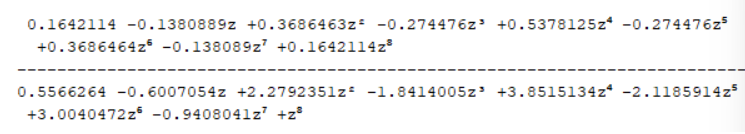
\includegraphics[width=\textwidth]{h_bp.png}
    \caption{Screenshot from SCILAB Console.}
\end{figure}

\subsection{Frequency Response}
The frequency response of the Elliptic Bandpass Filter with order N = 4 is provided on the next page.

\begin{figure}
    \centering
    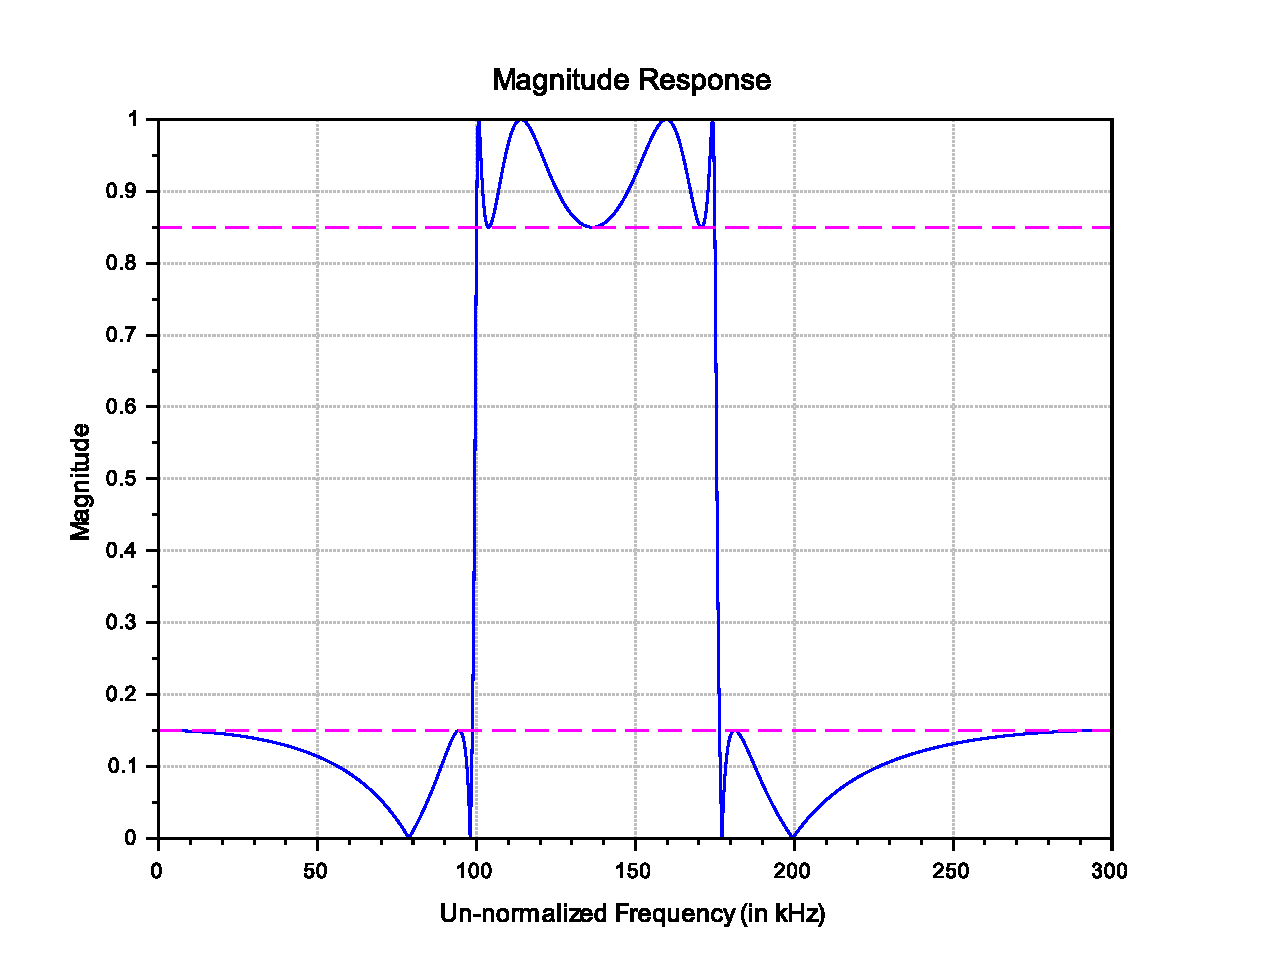
\includegraphics[scale=0.6]{mag_bp.pdf}
    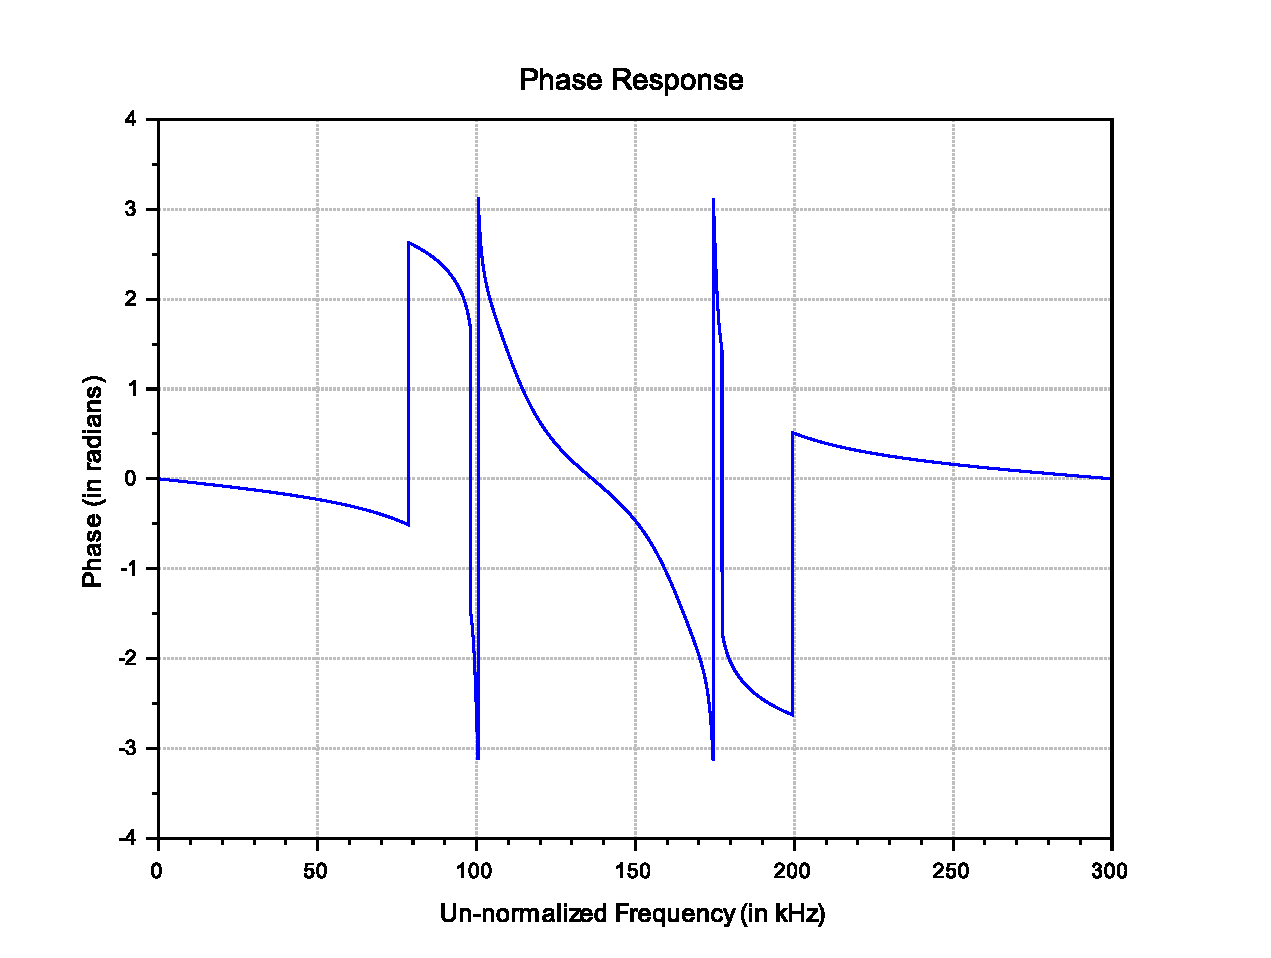
\includegraphics[scale=0.6]{phase_bp.pdf}
\end{figure}

\newpage

\section{Bandstop Filter Design}
\subsection{Un-normalized Discrete Time Filter}
\[q(m) = r(m) = 5\]
\begin{align*}
    BL(m) &= 20 + 3 q(m) + 11 r(m),\\
    &= 20 + 3(5) + 11(5)\\
    &= 90,\\
    BH(m) &= BL(m) + 40,\\
    &= 90 + 40\\
    &= 130.
\end{align*}
Therefore, the stopband edges are:
\begin{align*}
    f_{s1} &= 90 kHz,\\
    f_{s2} &= 130 kHz.
\end{align*}
The transition bandwidth is given to be\[\Delta_f = 5 kHz.\]
Therefore, the passband edges are:
\begin{align*}
    f_{p1} &= f_{s1} - \Delta_f = 85 kHz,\\
    f_{p2} &= f_{s2} + \Delta_f = 135 kHz.
\end{align*}

Now we can state the specifications of the discrete-time Bandstop filter.
\hline
\vspace{10pt}
\textbf{Specifications:}
\begin{itemize}
    \item Passband: 0 to 85 kHz and 135 kHz to 212.5 kHz (since $f_s$ = 425 kHz),
    \item Stopband: 90 kHz to 130 kHz,
    \item Passband and Stopband tolerance: 0.15,
    \item Passband and Stopband nature: Rippled.
\end{itemize}
\hline

\subsection{Normalized Digital Filter}
Given that our signal of interest is bandlimited to
\[f_b = 200 kHz,\]
to satisfy the Nyquist Criterion,
\[f_s > 2 f_b = 400 kHz.\]
Given sampling frequency is
\[f_s = 425 kHz > 400 kHz.\]
Hence, the Nyquist criterion is satisfied.

For normalizing the frequencies, we need to make the sampling frequency map to $2\pi$. Thus,
\[\omega = \frac{2\pi f}{f_s}\]

This gives us the normalized digital frequencies as follows:
\begin{table}[h]
    \centering
    \begin{tabular}{|c|c|}\hline
         Discrete time frequency&Normalized digital frequency\\
         $f$ (kHz)&$\omega$ (radians)\\\hline
         0&0\\\hline
         85&$\omega_{p1}$ = 1.2566371\\\hline
         90&$\omega_{s1}$ = 1.3305569\\\hline
         130&$\omega_{s2}$ = 1.9219155\\\hline
         135&$\omega_{p2}$ = 1.9958353\\\hline
         212.5&$\pi$\\\hline
    \end{tabular}
    \caption{Normalizing frequency.}
    \label{tab:1}
\end{table}

Now we can state the specifications of the digital Bandstop filter.
\newline
\hline
\vspace{10pt}
\textbf{Specifications:}
\begin{itemize}
    \item Passband: 0 to 1.2566371 and 1.9958353 to  $\pi$,
    \item Stopband: 1.3305569 to 1.9219155,
    \item Passband and Stopband tolerance: 0.15,
    \item Passband and Stopband nature: Rippled.
\end{itemize}
\hline

\subsection{Analog Bandstop Filter}
For converting the normalized digital specifications to the specifications for an analog filter of the same type (Bandstop), we use the bilinear transformation:
\[s = \frac{1-z^{-1}}{1+z^{-1}},\]
substituting the values of s and z, we get
\begin{align*}
    j\Omega &= \frac{1-e^{-j\omega}}{1+e^{-j\omega}} = \frac{e^{j\omega/2}-e^{-j\omega/2}}{e^{+j\omega/2}+e^{-j\omega/2}}\\
    &= \frac{2j\sin(\omega/2)}{2\cos(\omega/2)} = j\tan(\omega/2)\\
    \Omega &= \tan(\omega/2)
\end{align*}
This gives us the analog Bandstop frequencies as:
\begin{table}[h]
    \centering
    \begin{tabular}{|c|c|}\hline
         Normalized digital frequency&Analog frequency\\
         $\omega$ (radians)&$\Omega$\\\hline
         0&0\\\hline
         1.2566371&$\Omega_{p1}$ = 0.7265425\\\hline
         1.3305569&$\Omega_{s1}$ = 0.7845976\\\hline
         1.9219155&$\Omega_{s2}$ = 1.4312732\\\hline
         1.9958353&$\Omega_{p2}$ = 1.5502977\\\hline
         $\pi$&$\infty$\\\hline
    \end{tabular}
    \caption{Applying the bilinear transformation.}
    \label{tab:2}
\end{table}

Now we can state the specifications of the digital Bandstop filter.
\newline
\hline
\vspace{10pt}
\textbf{Specifications:}
\begin{itemize}
    \item Passband: 0 to 0.7265425 and 1.5502977 to $\infty$,
    \item Stopband: 0.7845976 to 1.4312732,
    \item Passband and Stopband tolerance: 0.15,
    \item Passband and Stopband nature: Rippled.
\end{itemize}
\hline

\subsection{Frequency Transformation}
We need to employ a frequency transformation to convert our Bandstop filter specifications into those of a lowpass filter. For this, we use the frequency transformation derived from the impedance of a parallel LC circuit:
\[s_L = \frac{Bs}{s^2 + \Omega_0^2},\]
where the subscript L stands for Lowpass. $\Omega_0$ is the resonant frequency and B is the bandwidth of the parallel LC circuit. Substituting the values of s$_L$ and s, we get
\begin{align*}
    j\Omega_L &= \frac{B(j\Omega)}{(j\Omega)^2 + \Omega_0^2}\\
    &= j\frac{B\Omega}{(-\Omega^2 + \Omega_0^2)}\\
    \Omega_L &= \frac{B\Omega}{\Omega_0^2 - \Omega^2}
\end{align*}
Now, we have two degrees of freedom, $\Omega_0$ and B. We also decide to follow the convention that the passband edge of the lowpass filter, in both the positive and negative half of the $\Omega_L$ axis, has a magnitude of one. In other words, we want $\Omega_{p1}$ and $\Omega_{p2}$ to map to +1 and -1 respectively on the $\Omega_L$ axis. To achieve this, we solve the following two equations
\[+1 = \frac{B\Omega_{p1}}{\Omega_0^2 - \Omega_{p1}^2}\]
and
\[-1 = \frac{B\Omega_{p2}}{\Omega_0^2 - \Omega_{p2}^2}\]
By equating $\Omega_0^2$ we get
\begin{align*}
    \Omega_{p1}^2 + B\Omega_{p1} &= \Omega_{p2}^2 - B\Omega_{p2}\\
    B(\Omega_{p2} + \Omega_{p1}) &= \Omega_{p2}^2 - \Omega_{p1}^2\\
    B &= \Omega_{p2} - \Omega_{p1}
\end{align*}
Substituting the value of B, we get
\begin{align*}
    \Omega_0^2 &= \Omega_{p1}^2 + (\Omega_{p2} - \Omega_{p1})\Omega_{p1}\\
    \Omega_0^2 &= \Omega_{p1}^2 + \Omega_{p2}\Omega_{p1} - \Omega_{p1}^2 = \Omega_{p2}\Omega_{p1}\\
    \Omega_0 &= \sqrt{\Omega_{p2}\Omega_{p1}}
\end{align*}
By substituting the value of $\Omega_{p1}$ and $\Omega_{p2}$, we get
\begin{align*}
    B &= 1.5502977 - 0.7265425 = 0.8237552\\
    \Omega_0 &= \sqrt{(1.5502977)(0.7265425)} = \sqrt{1.1263572} \approx 1.0612998
\end{align*}
\hline
\vspace{10pt}
\textbf{Transformation and Parameters}
\begin{itemize}
    \item Transformation:\[\Omega_L = \frac{B\Omega}{\Omega_0^2 - \Omega^2}\]
    \item Parameters:
    \begin{itemize}
        \item $\Omega_0$ = 1.0612998,
        \item B = 0.8237552
    \end{itemize}
\end{itemize}
\hline
\newpage
\subsection{Analog Lowpass Filter}
Substituting the values of $\Omega_o$ and B, we get the frequency transformation to be employed as:
\[\Omega_L = \frac{(0.8237552)\Omega}{(1.1263572) - \Omega^2}\]
This gives us the analog lowpass frequencies as:
\begin{table}[!h]
    \centering
    \begin{tabular}{|c|c|}\hline
         Analog frequency&Analog Lowpass Frequency\\
         $\Omega$ &$\Omega_L$\\\hline
         0$^+$&0$^+$\\\hline
         0.7265425&$\Omega_{Ls1}$ = 1.2653920\\\hline
         0.7845976&$\Omega_{Lp1}$ = 1\\\hline
         1.4312732&$\Omega_{Lp2}$ = -1\\\hline
         1.5502977&$\Omega_{Ls2}$ = -1.2785044\\\hline
         $\infty$&0$^-$\\\hline
    \end{tabular}
    \caption{Analog frequency transformation.}
    \label{tab:3}
\end{table}

The passband edge of the lowpass filter was specified to be one while employing the frequency transformation but, the stopband edge now has two possible values of which, we choose the more stringent value (the value with a smaller magnitude) since satisfying the stronger specifications will automatically satisfy the weaker specifications. Thus
\begin{align*}
    \Omega_p &= 1\\
    \Omega_s &= min(abs(\Omega_{Ls1}), abs(\Omega_{Ls1}))\\
    &= min(1.2653920, 1.2785044)\\
    \Omega_s &= 1.2653920
\end{align*}

Now we can state the specifications of the analog lowpass filter.
\newline
\hline
\vspace{10pt}
\textbf{Specifications:}
\begin{itemize}
    \item Passband: 0 to 1,
    \item Stopband: 1.2653920 to  $\infty$,
    \item Passband and Stopband tolerance: 0.15,
    \item Passband and Stopband nature: Rippled.
\end{itemize}
\hline
\newpage
\subsection{Elliptic Analog Lowpass Transfer Function}
The first step was finding the poles and zeros of the Elliptic analog lowpass transfer function using the functions provided in MATLAB.
\[N = 3,\]
\[\text{poles} = -0.1153 + j0.9936,\]
\[\text{additional pole} = -0.6232,\]
\[\text{zeros} = j1.2604.\]
Then, the Transfer function can be obtained using these poles and zeros and their complex conjugates along with the additional pole

\begin{figure}[h]
    \centering
    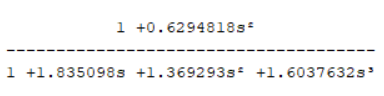
\includegraphics{h_lpf_bs.png}
    \caption{Screenshot from SCILAB Console.}
\end{figure}
Lowpass transfer function frequency response:

\begin{figure}[h]
    \begin{minipage}{0.49\linewidth}
        \centering
        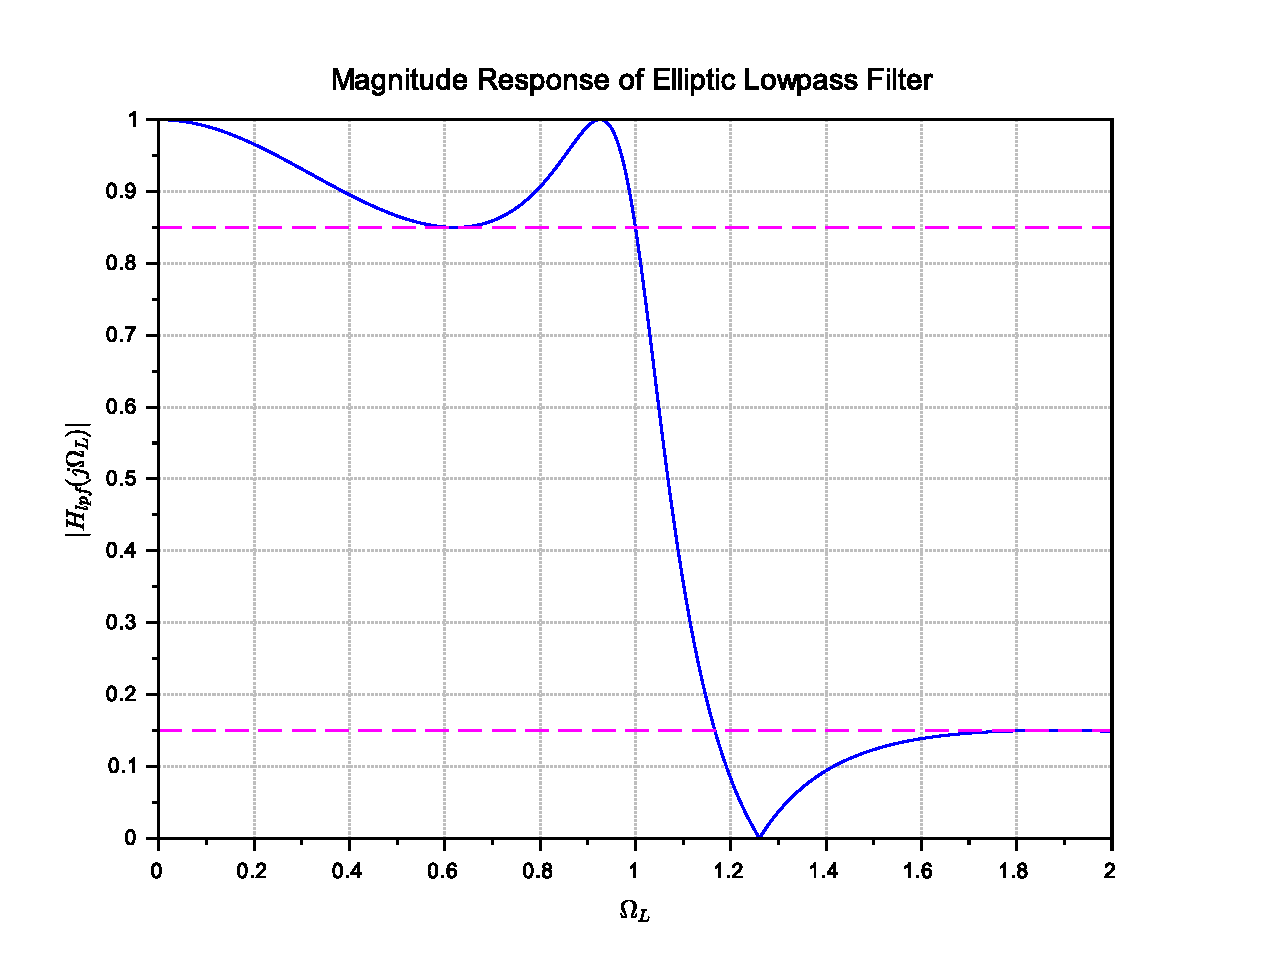
\includegraphics[scale=0.36]{mag_lpf_bs.pdf}
    \end{minipage}
    \begin{minipage}{0.49\linewidth}
        \centering
        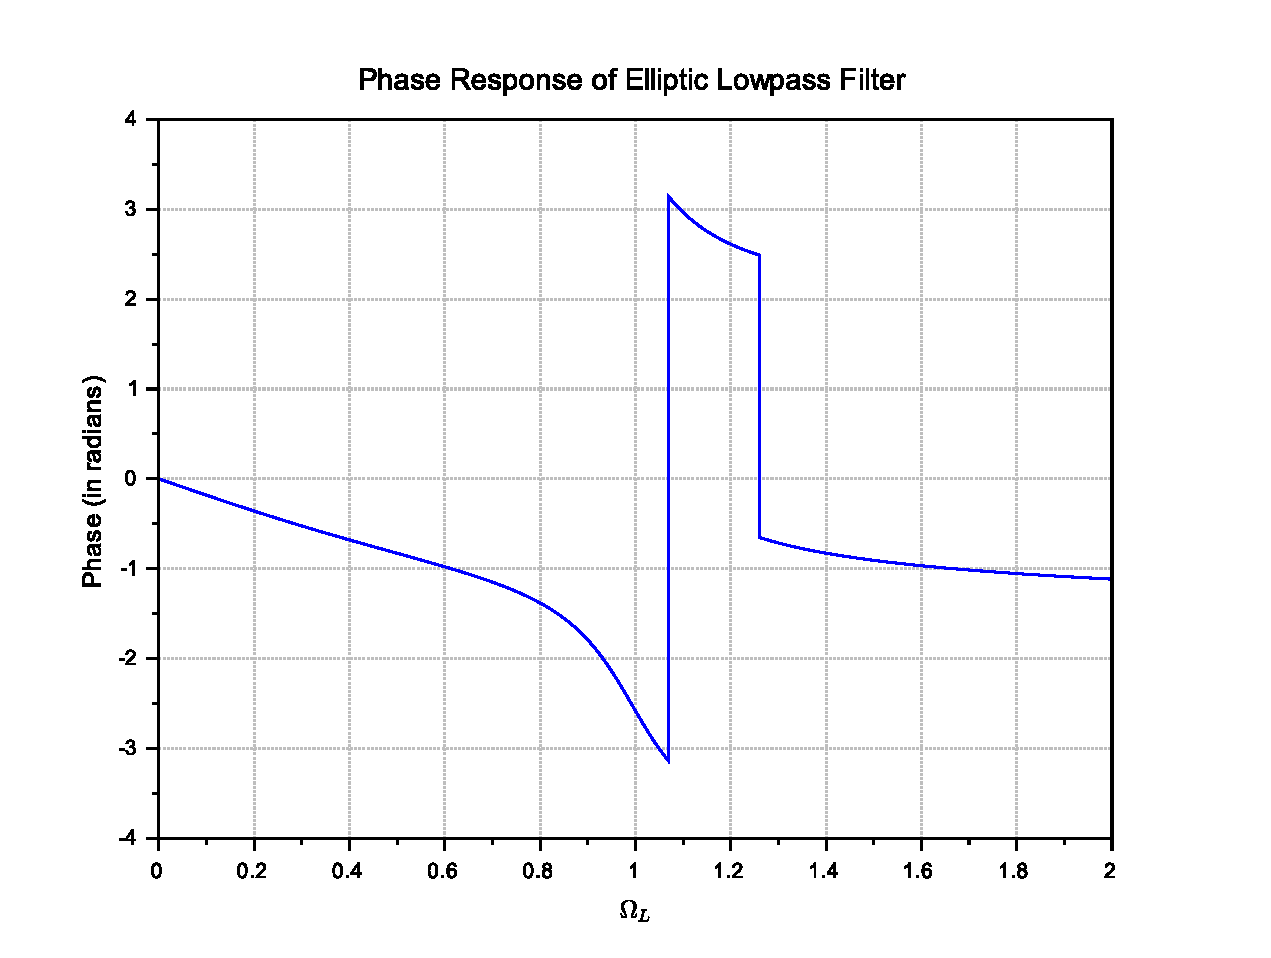
\includegraphics[scale=0.36]{phase_lpf_bs.pdf}
    \end{minipage}
\end{figure}

\subsection{Analog Bandstop Transfer Function}
This can be obtained by replacing s$_\text{L}$ with F(s), the frequency transformation that we had employed earlier:
\[s_L \leftarrow F(s) = \frac{Bs}{s^2 + \Omega_0^2}\]
\textbf{H$_{\text{analog, BSF}}\text{(s)}$}
\begin{figure}[h]
    \centering
    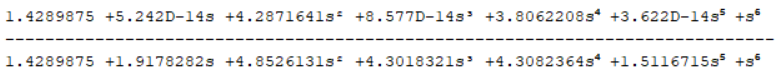
\includegraphics[width=\textwidth]{h_int_bs.png}
    \caption{Screenshot from SCILAB Console.}
\end{figure}

\subsection{Discrete Time Bandstop Transfer Function}
This can be obtained by applying the bilinear transformation to s:
\[s \leftarrow \frac{1 - z^{-1}}{1 + z^{-1}}\]
\textbf{H$_{\text{discrete time, BSF}}\text{(z)}$}
\begin{figure}[h]
    \centering
    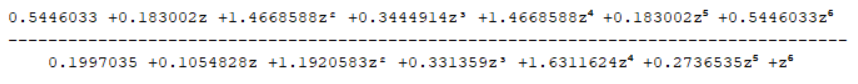
\includegraphics[width=\textwidth]{h_bs.png}
    \caption{Screenshot from SCILAB Console.}
\end{figure}


\subsection{Frequency Response}
The frequency response of the Elliptic Bandstop Filter with order N = 3 is provided on the next page.

\begin{figure}
    \centering
    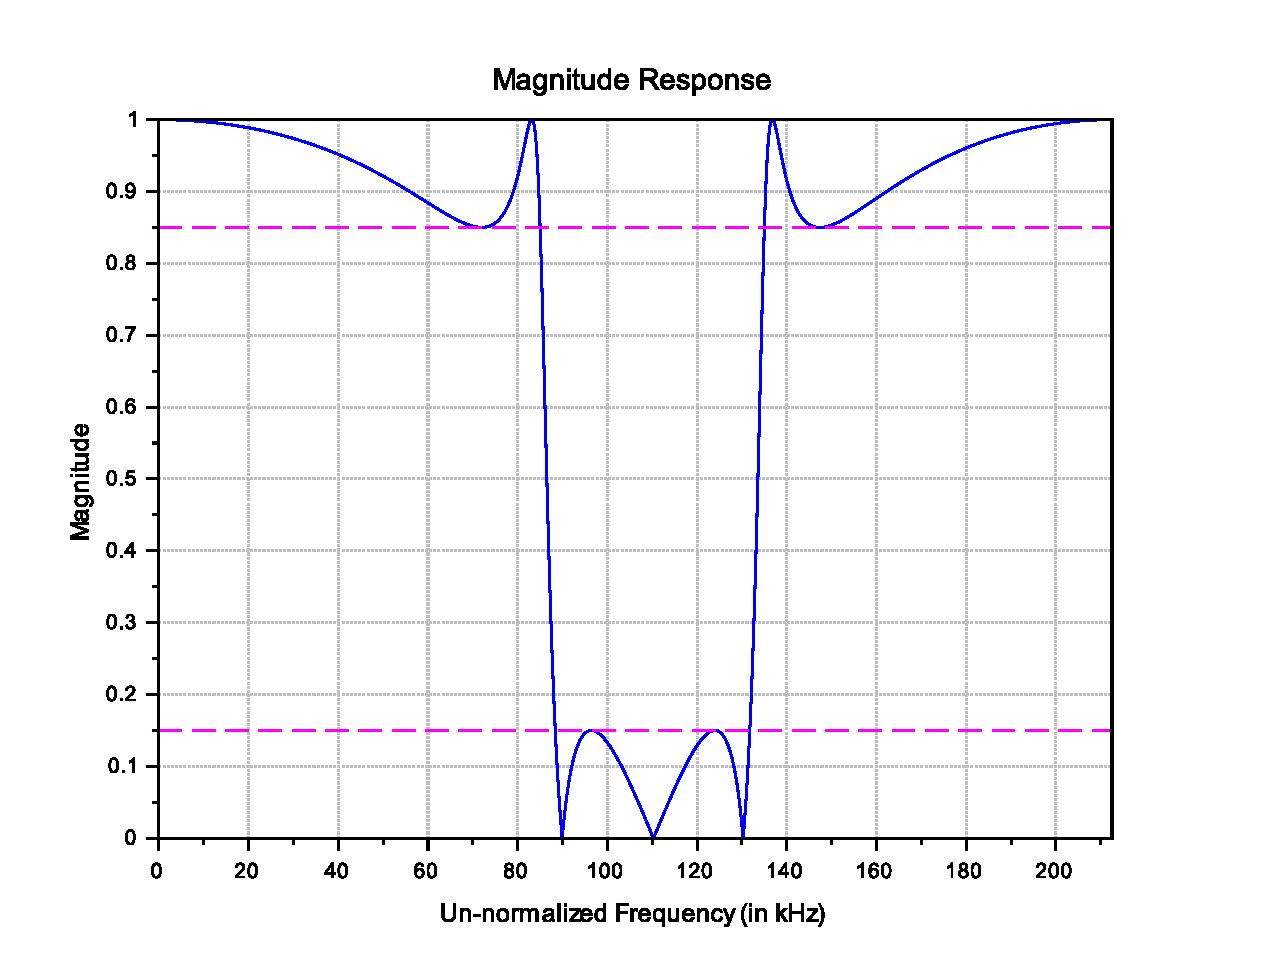
\includegraphics[scale=0.6]{mag_bs.pdf}
    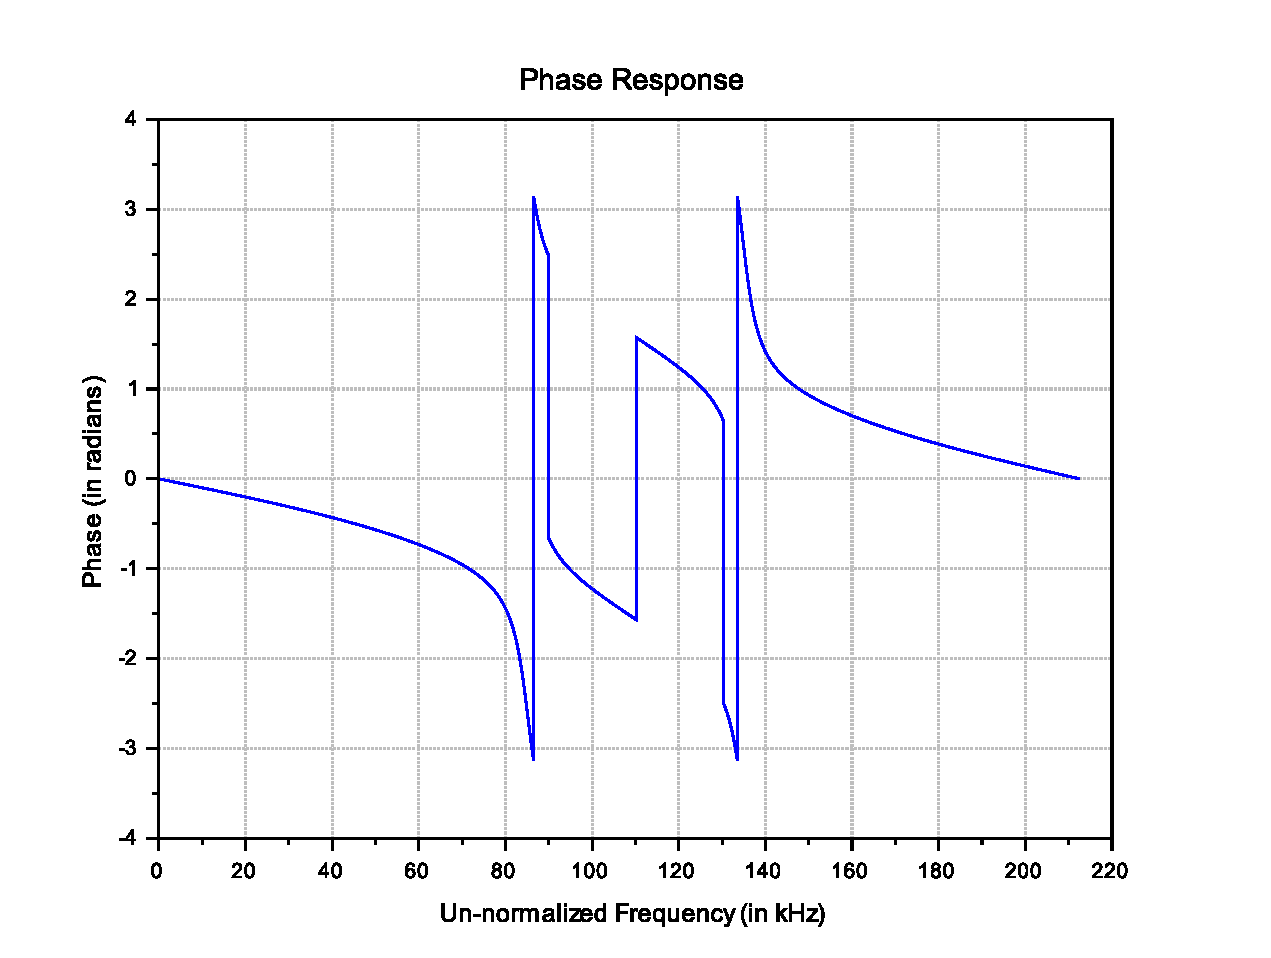
\includegraphics[scale=0.6]{phase_bs.pdf}
\end{figure}

\newpage
\section{References}
\href{https://www.ece.rutgers.edu/~orfanidi/ece521/notes.pdf}{Lecture Notes on Elliptic Filter Design - Rutgers ECE} by SJ Orfanidis.

\end{document}
